\chapter{MATERIALS AND METHODS}

\section{Study design}

This study employed a cross-sectional, secondary data analysis design, utilizing data from the Vietnam Multiple Indicator Cluster Survey (MICS6), conducted in 2020--2021 by the General Statistics Office of Vietnam in collaboration with UNICEF. MICS6 is a nationally representative household survey designed to generate disaggregated data on the situation of children and women, employing a two-stage stratified cluster sampling methodology \cite{unicef2022}.

The survey covered all 63 provinces and centrally-governed cities of Vietnam, with data collection conducted between January 2020 and June 2021. The Women's Questionnaire was administered through face-to-face interviews with all women aged 15--49 years residing in selected households, covering topics including reproductive health, child health, education, media exposure, and---critically for this study---knowledge of and experience with HPV vaccination.

\section{Study participants}

\subsection{Inclusion criteria}

\begin{itemize}
	\item Women aged 15--29 years (corresponding to MICS age groups WAGE 1--3) who completed the Women's Individual Questionnaire.
	\item Valid sampling weights, primary sampling unit (PSU), and stratification information available for survey-weighted analysis.
\end{itemize}

\subsection{Exclusion criteria}

\begin{itemize}
	\item Women with missing sampling weights (\texttt{wmweight}), PSU identifiers, or stratum indicators, as these preclude valid survey-weighted estimation.
	\item Records with indeterminate responses on both outcome variables (HPV awareness and vaccination status).
\end{itemize}

\begin{figure}[htbp]
\centering
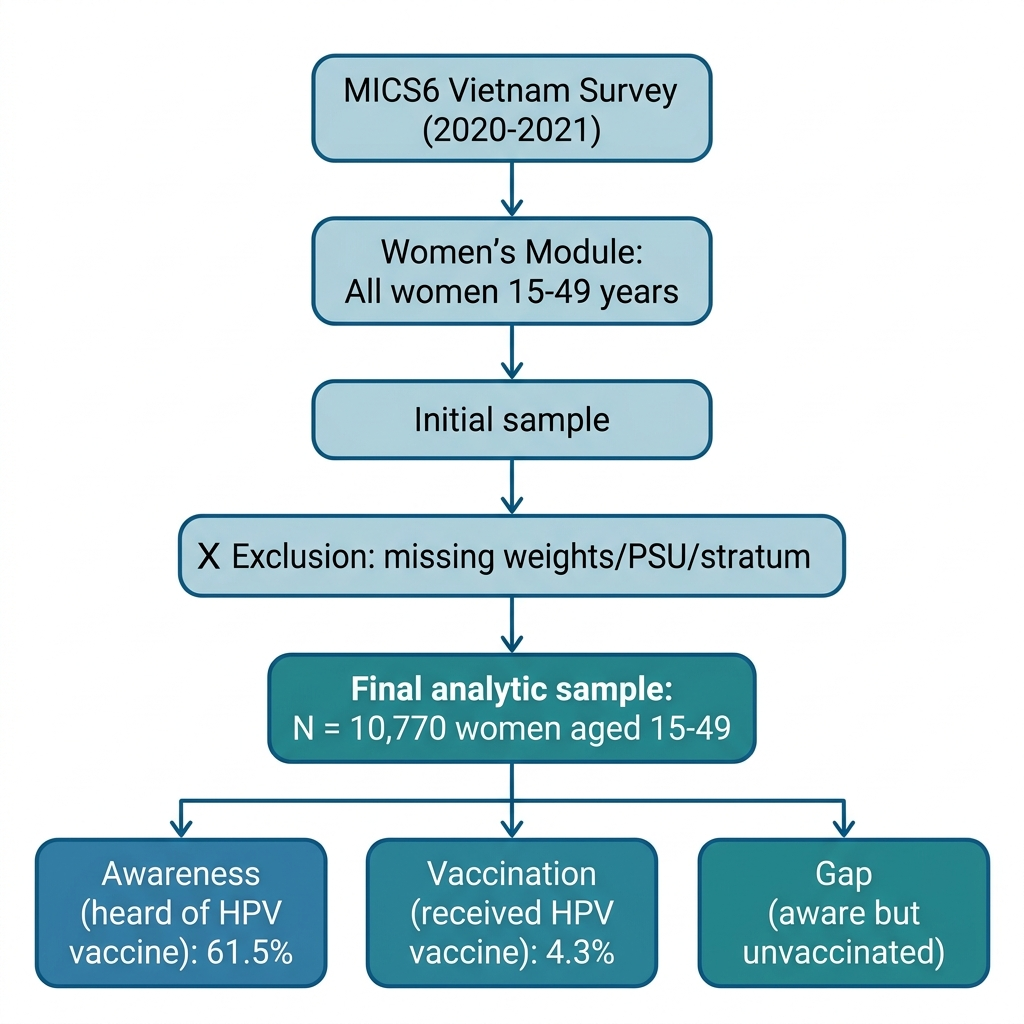
\includegraphics[width=0.82\textwidth]{Figures/study_design_flowchart.png}
\caption{Study design and participant selection flowchart. From the MICS6 Women's Module, the final analytic sample comprised 4,102 women aged 15--29 after excluding records with missing survey design variables.}
\label{fig:study_flowchart}
\end{figure}

\section{Sample size}

The analytic sample consisted of all eligible women from the MICS6 survey who met the inclusion criteria. After applying exclusion criteria, the final sample comprised \textbf{N~=~4,102} women aged 15--29 years. This sample size provides adequate statistical power for detecting inequality patterns and conducting multivariable regression and decomposition analyses. No additional sample size calculation was performed, as this study utilized the complete available dataset from a nationally representative survey.

\section{Study variables}

\subsection{Outcome variables}

Three binary outcome variables were constructed from the MICS6 cervical cancer prevention module:

\begin{enumerate}
	\item \textbf{HPV vaccine awareness} (\texttt{ccp5\_bin}): Derived from MICS item CCP5 (``Have you ever heard of HPV vaccination?''). Coded as 1~=~Yes, 0~=~No.
	
	\item \textbf{HPV vaccination status} (\texttt{ccp6\_bin}): Derived from MICS item CCP6 (``Have you ever received the HPV vaccine?''). Coded as 1~=~Yes, 0~=~No or Don't Know. Women who reported not having heard of HPV vaccination (CCP5~=~No) were classified as unvaccinated (CCP6~=~0), consistent with the MICS skip pattern.
	
	\item \textbf{Awareness--vaccination gap} (\texttt{gap}): Defined among aware women only (CCP5~=~Yes). Coded as 1 if the woman was aware but unvaccinated, 0 if aware and vaccinated. This variable captures the ``knowing--doing gap'' relevant to behavioral intervention design.
\end{enumerate}

\subsection{Explanatory variables}

Based on the conceptual framework (Section~1.6) and available MICS6 data, the following covariates were included:

\begin{table}[htbp]
\caption{Summary of explanatory variables used in the analysis}
\centering
\small
\begin{tabular}{|p{3.2cm}|p{4.2cm}|p{5.8cm}|}
\hline
\textbf{Variable} & \textbf{Categories} & \textbf{Operational Definition} \\
\hline
Age group (WAGE) & 15--19, 20--24, 25--29 & MICS standard 5-year age groups \\
\hline
Residence (area) & Urban, Rural & MICS household classification \\
\hline
Ethnicity (minority) & Kinh/Hoa (No), Ethnic minority (Yes) & MICS variable ethnicity2 \\
\hline
Marital status (MSTATUS) & Currently married/union, Formerly married, Never married & MICS marital status variable \\
\hline
Education (edu) & Primary or less, Lower secondary, Upper secondary+ & Collapsed from MICS welevel \\
\hline
Wealth quintile (ses5) & Q1 (poorest) to Q5 (richest) & MICS wealth index quintiles \\
\hline
Health insurance (insu) & Insured (No), Uninsured (Yes) & MICS insurance variable \\
\hline
Mass media exposure (mme) & No, Yes & Any exposure to newspaper, radio, or TV \\
\hline
ICT exposure (ict) & No, Yes & Any use of computer, internet, or mobile \\
\hline
Decision autonomy (dvindex) & Low (No), High (Yes) & All 5 DV1 items answered ``jointly'' \\
\hline
Sexual experience (sb1n) & No, Yes & Ever had sexual intercourse (SB1) \\
\hline
\end{tabular}
\label{tab:variables}
\end{table}

\section{Data analysis}

All analyses were performed using Stata version 17 (StataCorp LLC, College Station, TX) with the \texttt{svy:} prefix to account for the complex survey design (stratification, clustering, and sampling weights). The analytical strategy followed a sequential five-step approach:

\begin{figure}[htbp]
\centering
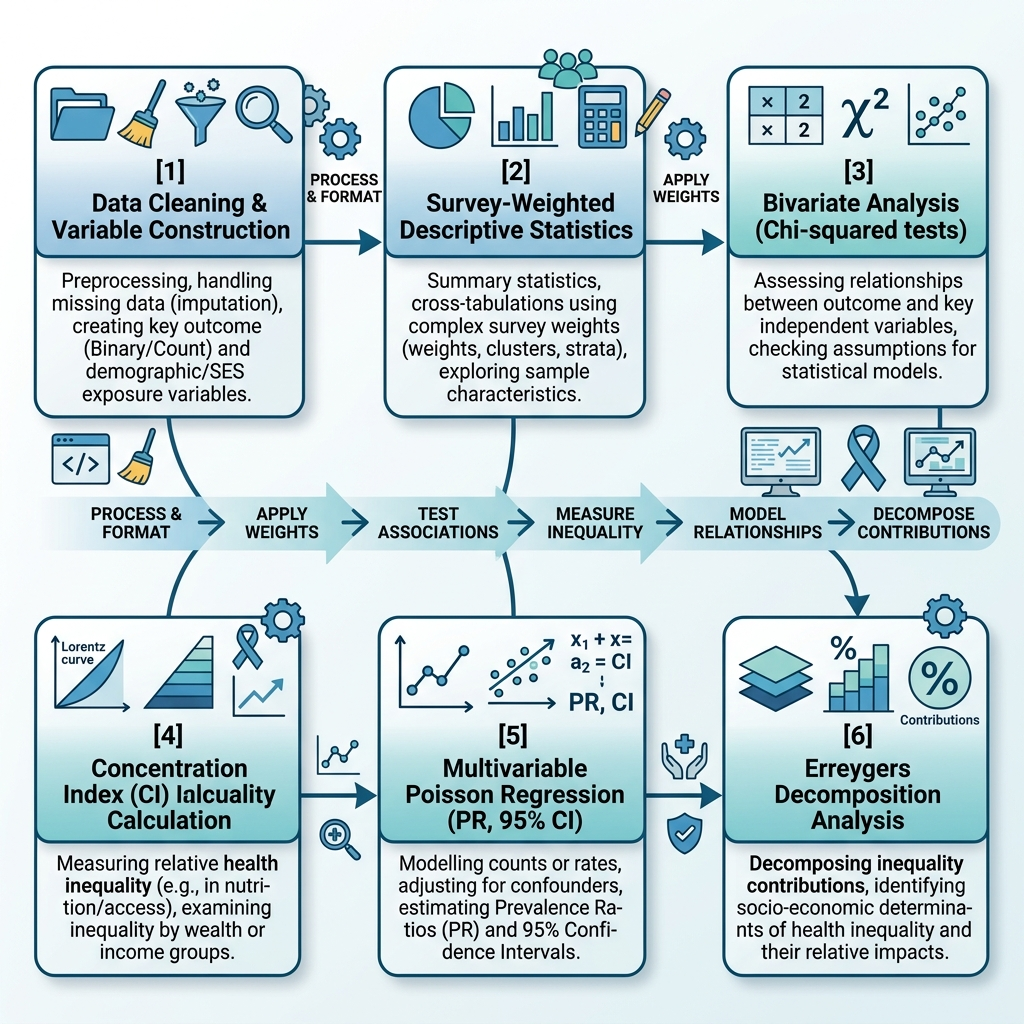
\includegraphics[width=0.85\textwidth]{Figures/analysis_pipeline.png}
\caption{Statistical analysis pipeline. The six-stage analytical approach progresses from data preparation through descriptive analysis, bivariate testing, inequality quantification, multivariable modeling, and decomposition.}
\label{fig:analysis_pipeline}
\end{figure}

\subsection{Step 1: Descriptive statistics}

Survey-weighted proportions with 95\% confidence intervals were computed for all outcome and explanatory variables to characterize the study population and estimate the prevalence of HPV awareness and vaccination.

\subsection{Step 2: Bivariate analysis}

The association between each explanatory variable and the outcome variables was assessed using survey-weighted Pearson chi-squared tests with Rao--Scott corrections for complex survey design. Row percentages with 95\% confidence intervals were reported. Statistical significance was set at $\alpha = 0.05$.

\subsection{Step 3: Concentration index}

The Wagstaff concentration index (CI) provides a rigorous econometric quantification of socioeconomic inequality in health outcomes \cite{wagstaff2000}. In this study, the standard CI was formulated mathematically as both the scaled covariance between the health outcome and the fractional rank in the living standards distribution, and geometrically as the area integral:

\begin{equation}
CI = \frac{2}{\mu} \mathrm{cov}(y_i,\, r_i) = \frac{2}{\mu} \int_0^1 \bigl( y(r) - \mu \bigr) r \,dr
\end{equation}

\noindent where $y_i$ represents the binary outcome for individual $i$, $r_i$ is the continuous fractional rank in the socioeconomic distribution (household wealth score), and $\mu$ is the survey-weighted population mean of the outcome. Geometrically, the CI equals twice the area between the concentration curve and the line of equality. A positive CI ($0 < CI \le 1$) indicates pro-rich inequality, whereas a negative CI ($-1 \le CI < 0$) signifies pro-poor concentration.

\subsection{Step 4: Multivariable Poisson regression}

Because the prevalence of HPV awareness exceeded the 10\% threshold, logistic regression would mathematically yield odds ratios that severely overestimate the true relative risk \cite{barros2003}. Consequently, we employed modified Poisson regression---a generalized linear model (GLM) featuring a logarithmic link function and a Poisson distribution---to directly estimate adjusted prevalence ratios (PR). To correct for the violation of the Poisson assumption (variance equal to the mean) inherent in binary data, robust Huber-White sandwich variance estimators were applied. The formal model specification is:

\begin{equation}
\log\bigl[E(Y_i \mid \mathbf{X}_i)\bigr] = \mathbf{X}_i^\top \boldsymbol{\beta} \quad \text{with robust variance:} \quad \widehat{\mathbf{V}}(\hat{\boldsymbol{\beta}}) = \mathbf{D}^{-1} \mathbf{M} \mathbf{D}^{-1}
\end{equation}

\noindent where $E(Y_i \mid \mathbf{X}_i)$ is the expected probability of the outcome given the covariate vector $\mathbf{X}_i$, and $\boldsymbol{\beta}$ is the vector of coefficients. The exponentiated coefficients ($\exp(\beta_k)$) provide the direct prevalence ratios. The matrix $\mathbf{D}$ represents the expected information matrix, and $\mathbf{M}$ is the outer product of the empirical gradients. The reference categories were: age 25--29, currently married, upper secondary+ education, Q5 (richest), and the absence category for binary covariates.

A sensitivity analysis using logistic regression (yielding odds ratios) was conducted to assess the robustness of findings.

\subsection{Step 5: Erreygers decomposition}

A fundamental mathematical limitation of the standard Wagstaff CI is that its absolute bounds contract as the mean of the binary outcome deviates from 0.5, distorting comparative analyses across populations. To circumvent this scale dependence, we utilized the Erreygers Concentration Index ($ECI$), which restores the normative limits to $[-1, 1]$ via the transformation:

\begin{equation}
ECI(y) = 4 \mu (1 - \mu) CI(y)
\end{equation}

The $ECI$ was subsequently decomposed to isolate the specific econometric contributions of each explanatory variable \cite{erreygers2009}. Given a generalized linear mapping via a probit link, the exact contribution of each covariate $k$ is calculated as the product of its partial marginal effect, its weighted mean, and its own concentration index:

\begin{equation}
\text{Contribution}_k = 4 \cdot \left( \frac{\partial E(y \mid \mathbf{x})}{\partial x_k} \right) \cdot \bar{x}_k \cdot CI_{x_k} = 4 \cdot \beta_k^{AME} \cdot \bar{x}_k \cdot CI_{x_k}
\label{eq:erreygers_contrib}
\end{equation}

\noindent where $\beta_k^{AME}$ is the average marginal effect from a probit model, $\bar{x}_k$ is the weighted mean of the covariate, and $CI_{x_k}$ is the Erreygers-corrected concentration index of the covariate with respect to the wealth ranking. The percentage contribution of each covariate was computed as:

\begin{equation}
\text{Percentage}_k = \frac{\text{Contribution}_k}{ECI_{\text{total}}} \times 100
\label{eq:pct_contrib}
\end{equation}

Decomposition was performed separately for each of the three outcome variables: awareness, vaccination, and the awareness--vaccination gap.

\subsection{Step 6: Stratified and sensitivity analyses}

Additional analyses included:
\begin{itemize}
	\item \textbf{Stratified regression} by urban/rural residence to examine whether determinants differed between settings.
	\item \textbf{Crude (unadjusted) Poisson regression} for each variable individually to compare crude and adjusted prevalence ratios.
	\item \textbf{Logistic regression sensitivity analysis} to verify that key findings were robust to the choice of link function.
	\item \textbf{Gap model}: Poisson regression among aware women to identify factors associated with failure to translate awareness into vaccination action.
\end{itemize}

\section{Ethical considerations}

The MICS6 survey protocol was approved by the Institutional Review Board of the General Statistics Office of Vietnam and received ethical clearance from UNICEF's Division of Data, Analytics, Planning, and Monitoring. Written informed consent was obtained from all individual respondents prior to interview participation. For respondents under the age of 18, parental/guardian consent was also obtained.

This study constitutes a secondary analysis of de-identified, publicly available survey data. No direct contact with human subjects occurred. All data were accessed and analyzed in compliance with the MICS data use agreement.